\documentclass{article}

\usepackage{multirow}
\usepackage{dcolumn}
\newcolumntype{2}{D{.}{}{2.0}}
\usepackage{graphicx}
\usepackage{fullpage,latexsym,picinpar,amsmath,amsfonts,graphicx}
\usepackage{qtree,polynom}
\usepackage{systeme}

           

%%%%%%%%%%%%%%%%%%%%%%%%%%%%%%%%%%%%%%%%%%%%%%%%%%%%%%%%%%%%%%%%%%%%%%%%%%%%%%%%%%%
%%%%%%%%%%%  LETTERS 
%%%%%%%%%%%%%%%%%%%%%%%%%%%%%%%%%%%%%%%%%%%%%%%%%%%%%%%%%%%%%%%%%%%%%%%%%%%%%%%%%%%

\newcommand{\barx}{{\bar x}}
\newcommand{\bary}{{\bar y}}
\newcommand{\barz}{{\bar z}}
\newcommand{\bart}{{\bar t}}

\newcommand{\bfP}{{\bf{P}}}

%%%%%%%%%%%%%%%%%%%%%%%%%%%%%%%%%%%%%%%%%%%%%%%%%%%%%%%%%%%%%%%%%%%%%%%%%%%%%%%%%%%
%%%%%%%%%%%%%%%%%%%%%%%%%%%%%%%%%%%%%%%%%%%%%%%%%%%%%%%%%%%%%%%%%%%%%%%%%%%%%%%%%%%
                                                                                
\newcommand{\parend}[1]{{\left( #1  \right) }}
\newcommand{\spparend}[1]{{\left(\, #1  \,\right) }}
\newcommand{\angled}[1]{{\left\langle #1  \right\rangle }}
\newcommand{\brackd}[1]{{\left[ #1  \right] }}
\newcommand{\spbrackd}[1]{{\left[\, #1  \,\right] }}
\newcommand{\braced}[1]{{\left\{ #1  \right\} }}
\newcommand{\leftbraced}[1]{{\left\{ #1  \right. }}
\newcommand{\floor}[1]{{\left\lfloor #1\right\rfloor}}
\newcommand{\ceiling}[1]{{\left\lceil #1\right\rceil}}
\newcommand{\barred}[1]{{\left|#1\right|}}
\newcommand{\doublebarred}[1]{{\left|\left|#1\right|\right|}}
\newcommand{\spaced}[1]{{\, #1\, }}
\newcommand{\suchthat}{{\spaced{|}}}
\newcommand{\numof}{{\sharp}}
\newcommand{\assign}{{\,\leftarrow\,}}
\newcommand{\myaccept}{{\mbox{\tiny accept}}}
\newcommand{\myreject}{{\mbox{\tiny reject}}}
\newcommand{\blanksymbol}{{\sqcup}}
                                                                                                                         
\newcommand{\veps}{{\varepsilon}}
\newcommand{\Sigmastar}{{\Sigma^\ast}}
                           
\newcommand{\half}{\mbox{$\frac{1}{2}$}}    
\newcommand{\threehalfs}{\mbox{$\frac{3}{2}$}}   
\newcommand{\domino}[2]{\left[\frac{#1}{#2}\right]}  

%%%%%%%%%%%% complexity classes

\newcommand{\PP}{\mathbb{P}}
\newcommand{\NP}{\mathbb{NP}}
\newcommand{\PSPACE}{\mathbb{PSPACE}}
\newcommand{\coNP}{\textrm{co}\mathbb{NP}}
\newcommand{\DLOG}{\mathbb{L}}
\newcommand{\NLOG}{\mathbb{NL}}
\newcommand{\NL}{\mathbb{NL}}

%%%%%%%%%%% decision problems

\newcommand{\PCP}{\sc{PCP}}
\newcommand{\Path}{\sc{Path}}
\newcommand{\GenGeo}{\sc{Generalized Geography}}

\newcommand{\malytm}{{\mbox{\tiny TM}}}
\newcommand{\malycfg}{{\mbox{\tiny CFG}}}
\newcommand{\Atm}{\mbox{\rm A}_\malytm}
\newcommand{\complAtm}{{\overline{\mbox{\rm A}}}_\malytm}
\newcommand{\AllCFG}{{\mbox{\sc All}}_\malycfg}
\newcommand{\complAllCFG}{{\overline{\mbox{\sc All}}}_\malycfg}
\newcommand{\complL}{{\bar L}}
\newcommand{\TQBF}{\mbox{\sc TQBF}}
\newcommand{\SAT}{\mbox{\sc SAT}}

%%%%%%%%%%%%%%%%%%%%%%%%%%%%%%%%%%%%%%%%%%%%%%%%%%%%%%%%%%%%%%%%%%%%%%%%%%%%%%%%%%%
%%%%%%%%%%%%%%% for homeworks
%%%%%%%%%%%%%%%%%%%%%%%%%%%%%%%%%%%%%%%%%%%%%%%%%%%%%%%%%%%%%%%%%%%%%%%%%%%%%%%%%%%

\newcommand{\student}[2]{%
{\noindent\Large{ \emph{#1} SID {#2} } \hfill} \vskip 0.1in}

\newcommand{\assignment}[1]{\medskip\centerline{\large\bf CS 111 ASSIGNMENT {#1}}}

\newcommand{\duedate}[1]{{\centerline{due {#1}\medskip}}}     

\newcounter{problemnumber}                                                                                 

\newenvironment{problem}{{\vskip 0.1in \noindent
              \bf Problem~\addtocounter{problemnumber}{1}\arabic{problemnumber}:}}{}

\newcounter{solutionnumber}

\newenvironment{solution}{{\vskip 0.1in \noindent
             \bf Solution~\addtocounter{solutionnumber}{1}\arabic{solutionnumber}:}}
				{\ \newline\smallskip\lineacross\smallskip}

\newcommand{\lineacross}{\noindent\mbox{}\hrulefill\mbox{}}

\newcommand{\decproblem}[3]{%
\medskip
\noindent
\begin{list}{\hfill}{\setlength{\labelsep}{0in}
                       \setlength{\topsep}{0in}
                       \setlength{\partopsep}{0in}
                       \setlength{\leftmargin}{0in}
                       \setlength{\listparindent}{0in}
                       \setlength{\labelwidth}{0.5in}
                       \setlength{\itemindent}{0in}
                       \setlength{\itemsep}{0in}
                     }
\item{{{\sc{#1}}:}}
                \begin{list}{\hfill}{\setlength{\labelsep}{0.1in}
                       \setlength{\topsep}{0in}
                       \setlength{\partopsep}{0in}
                       \setlength{\leftmargin}{0.5in}
                       \setlength{\labelwidth}{0.5in}
                       \setlength{\listparindent}{0in}
                       \setlength{\itemindent}{0in}
                       \setlength{\itemsep}{0in}
                       }
                \item{{\em Instance:\ }}{#2}
                \item{{\em Query:\ }}{#3}
                \end{list}
\end{list}
\medskip
}

%%%%%%%%%%%%%%%%%%%%%%%%%%%%%%%%%%%%%%%%%%%%%%%%%%%%%%%%%%%%%%%%%%%%%%%%%%%%%%%%%%%
%%%%%%%%%%%%% for quizzes
%%%%%%%%%%%%%%%%%%%%%%%%%%%%%%%%%%%%%%%%%%%%%%%%%%%%%%%%%%%%%%%%%%%%%%%%%%%%%%%%%%%

\newcommand{\quizheader}{ {\large NAME: \hskip 3in SID:\hfill}
                                \newline\lineacross \medskip }


%%%%%%%%%%%%%%%%%%%%%%%%%%%%%%%%%%%%%%%%%%%%%%%%%%%%%%%%%%%%%%%%%%%%%%%%%%%%%%%%%%%
%%%%%%%%%%%%% for final
%%%%%%%%%%%%%%%%%%%%%%%%%%%%%%%%%%%%%%%%%%%%%%%%%%%%%%%%%%%%%%%%%%%%%%%%%%%%%%%%%%%

\newcommand{\namespace}{\noindent{\Large NAME: \hfill SID:\hskip 1.5in\ }\\\medskip\noindent\mbox{}\hrulefill\mbox{}}



\begin{document}
\centerline{Itzel Gonzalez SID: 861304050 and Jiunn Siow SID:86119666}
\centerline{\large \bf CS/MATH111 ASSIGNMENT 3}
%\centerline{due Wednesday, May 15}

\vskip 0.2in
%\noindent{\bf Individual assignment:} Problems 1 and 2.

%\noindent{\bf Group assignment:} Problems 1,2 and 3.

\vskip 0.1in

%%%%%%%%%%%%%%%%%%%%%%%%%%%%

\newcommand{\ttA}{\texttt{A}}
\newcommand{\ttB}{\texttt{B}}
\newcommand{\ttC}{\texttt{C}}
\newcommand{\ttE}{\texttt{E}}
\newcommand{\ttF}{\texttt{F}}

\begin{problem}
Strings of length $n$ are composed of the following strings: $\tt1$, $\tt2\tt2$, $\tt2\tt3$, $\tt3\tt2$, $\tt3\tt3$,
$\tt4\tt4\tt5$ and $\tt5\tt4\tt4$. Let $S_n$ be the number of strings of length $n$ that can
be formed in this way. For example, for $n=3$, we can form the following strings:
%
\begin{align*}
\tt1\tt1\tt1
,
\tt1\tt2\tt2  , \tt1\tt2\tt3  , \tt1\tt3\tt2  , \tt1\tt3\tt3
,
\tt2\tt2\tt1  , \tt2\tt3\tt1  , \tt3\tt2\tt1  , \tt3\tt3\tt1 
,
\tt4\tt4\tt5 , \tt5\tt4\tt4
\end{align*}
%
and thus $S_3 = 11$. (Note that $S_0 = 1$, because the
empty string satisfies the condition.)

\smallskip
\noindent (a) Derive a recurrence relation for the numbers $S_n$. Justify it.
\\

\Tree[.{Empty String}\\{S_n} 1\\S_{n-1} 
[.2 {(2,2)}\\S_{n-2} {(3,2)}\\S_{n-2} ] 
[.3 {(2,3)}\\S_{n-2} {(3,3)}\\S_{n-2} ]
445\\S_{n-3}
544\\S_{n-3}
]
\\
\text{In order to find the recurrence, we need to satisfy all the conditions which is that the string contains substrings }
\\
\text{ $\tt1$, $\tt2\tt2$, $\tt2\tt3$, $\tt3\tt2$, $\tt3\tt3$, $\tt4\tt4\tt5$,and $\tt5\tt4\tt4$. }
\text{We start with an $S_n$ or an empty string and then move on to the first case $S_{n-1}$}
\\
\text{Only $1$ satisfies the condition for $S_{n-1}$ and so we end the recursive case there.}
\\
\text{Next, we go to the 2nd character before the end and we find}
\text{all the cases containing the sub-strings with 2 and 3}
\\
\text{Finally, we go to the 3rd character before the end and we find}
\text{all the cases containing the sub-strings with 544 and 455}
\\
\text{We have accounted for all sub-strings that we have to put into our main string}
\\
\text{Adding all cases, the recurrence relation is $S_n = S_{n-1} + 4\cdot S_{n-2} + 2\cdot S_{n-3}$ for $n\geq3$ }
\\
\text{The Initial Conditions are: $S_0 = 1$,$S_1 = 1$, $S_2 = 5$, $S_3 = 11$}
\\
\smallskip
\noindent 
\pagebreak
\\(b) \textbf{Extra credit}. Let $P_n$ be the number of strings of length $n$ that can
be formed from the given strings,  considering that four 1's cannot be next to each other. (The substring 1111 is not allowed.) Derive a recurrence relation for the numbers $P_n$. Justify it.

Initial Conditions are:
$S_0 = 1$,$S_1 = 1$, $S_2 = 5$, $S_3 = 11$
\begin{figure}[h]
  \centering
  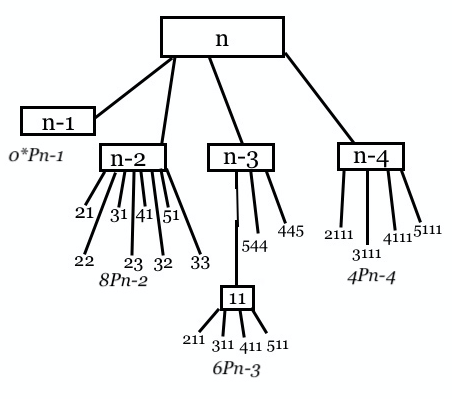
\includegraphics[width=70mm,,scale=1.5]{1.png}
\end{figure}\\
\text{Justification: For n-1, there are no options that can satisfy the condition so there are} 0*P_{n-1} 
\text{ options.}\\
\text{For n-2, the options are the given strings 22, 23, 32, 22 plus the conditions 21, 31, 41, and 51 because the strings}\\
\text{can be concatenated. Therefore we have } 8*P_{n-2}\text{. For n-3, we have the given strings 544, 445 and can concatenate} \\
\text{2, 3, 4, and 5 to the possible ending string 11. Therefore we have } 6*P_{n-3}
\text{. For n-4, we cannot have 1111 which is}\\
\text{the condition we were given. Therefore we must concatenate to get the 2111, 3111, 4111, and 5111 given strings}\\
\text{544, 445 and can concatenate 2, 3, 4, and 5 to the possible ending string 11. Therefore we have } 4*P_{n-4}\\\\
\text{When we add them together we get the final Recurrence Equation:}\\
\centerline{P_{n} = 8*P_{n-2} + 6*P_{n-3} + 4*P_{n-4}}


%\noindent (b) Find the formula for the numbers $S_n$ by solving this recurrence. Show your work.
\end{problem}

%%%%%%%%%%%%%%%%%%%%%%%%%%%%
\pagebreak
\begin{problem}
Solve the following recurrence equation:
\smallskip
\begin{align*}
	S_n &= S_{n-1} + 4S_{n-2} + 2S_{n-3}
	\\
	S_0 &= 1
	\\
	S_1 &= 1
	\\
	S_2 &= 5
\end{align*}

\noindent Show your work (all steps: the characteristic polynomial and its roots, the general solution, 
using the initial conditions to compute the final solution.)
\end{problem}
\\
\begin{alignat*}{2}
    & x^3 = x^2 +4\cdot x + 2
    && \hspace{20} \text{We get out characteristic polynomial first}
    \\
    & 0= x^3- x^2 - 4\cdot x -2
    && \hspace{20} \text{ We get possible roots 1,-1,2 and -2 by diving the lowest coefficient}
    \\
    & 0 = -1^3 - -1^2 +4 -2
    && \hspace{20} \text{Only $-1$ is the only root that works}
    \\
    & 0 = 0
    &&
\end{alignat*}
\text{We then do synthetic division with the root we just found}
\\
\polylongdiv{X^3-X^2-4X-2}{X+1}
\\
\text{We use quadratic formula to find the other roots}
\text{$x=\frac{-2\pm\sqrt{2^2+4*1*2}}{2*1}$}
\\
\text{The final roots we get are $1$,$1-\sqrt{3}$ and $1 +\sqrt{3}$}
\\
\text{Our general form equation is $S_n =(-1)^n\cdot\alpha_1 + (1+\sqrt{3})^n\cdot\alpha_2+(1-\sqrt{3})^n\cdot\alpha_3$ }
\\
\text{Setting up our initial conditions and systems of linear equations}
\[
\systeme*{1=\alpha_1 + \alpha_2 + \alpha_3,1=-\alpha_1 + (1+\sqrt{3})\alpha_2 + (1-\sqrt{3})\alpha_3,5=\alpha_1 + (1+\sqrt{3})^2\alpha_2 + (1-\sqrt{3})^2\alpha_3}
\]
\text{We get roots $\alpha_1 = 1$,$\alpha_2 = \frac{1}{\sqrt{3}}$,$\alpha_3 = -\frac{1}{\sqrt{3}}$}
\\
\text{The final solution is $S_n =(-1)^n + (1+\sqrt{3})^n\cdot\frac{1}{\sqrt{3}} - (1-\sqrt{3})^n\cdot\frac{1}{\sqrt{3}}$}
%%%%%%%%%%%%%%%%%%%%%%%%%%%%
\pagebreak
\begin{problem}
Solve the following recurrence equation:
%
\begin{eqnarray*}
        D_n &=& 4D_{n-1} -8 D_{n-3} + 2n+3\\
        D_0 &=& 0 \\
        D_1 &=& 1 \\
		D_2 &=& 1
\end{eqnarray*}
%
Show your work (all steps: the associated homogeneous equation,
the characteristic polynomial and its
roots, the general solution of the homogeneous
equation, computing a particular solution,
the general solution of the non-homogeneous equation,
using the initial conditions to compute the final solution.)
\end{problem}
\\\\
    Homogeneous Equation:\hspace{70} $D_n^{(h)} = 4D_{n-1} -8 D_{n-3}$
    \\\\
    Characteristic Polynomial:\hspace{75} $x^3- x^2 -8 = 0$
    \\\\
    To find possible roots 2, we use Rational Root Test along with Descartes' Rule of Signs. We use synthetic division with possible root 2:
    
    \[
    \renewcommand\arraystretch{1.5}
    \setlength\doublerulesep{0pt}
    \begin{array}{rrrrr}
    \multicolumn{1}{r|}{2}  & 1 & {-4} &0 & 8\\\cline{2-5}
     &  & {2} & {-4}& {-8}\\\cline{2-5}
     & 1 & {-2} & {-4}& 0
    \end{array}
    \]
    This gives us: $$(x - 2)(x^2 - 2x -4) = 0$$
    Using Quadratic Formula: 
    $$x=\frac{2\pm\sqrt{2^2-4(-4)}}{2} =\frac{2\pm\sqrt{20}}{2} =\frac{2\pm2\sqrt{5}}{2} ={1\pm\sqrt{5}}$$
    All roots are: 2, $ 1 \pm \sqrt{5}$\\
    Therefore, General Solution of Homogeneous Equation: $$D_n^{(h)} = (2)^n\cdot\alpha_1 + (1+\sqrt{5})^n\cdot\alpha_2+(1-\sqrt{5})^n\cdot\alpha_3$$
    \\
    Now we compute Particular Solution:\hspace{20} $$D_n = 2n + 3$$
    $$D_n^{(p)} = P_1n + P_0$$
    \\
    We plug into our equation as follows:
    \begin{align*}
    &P_1n + P_0 = 4(P_1(n-1) + P_0) - 8(P_1(n-3) + P_0) + 2n +3\\
    &P_1n + P_0 = 4P_1n-4P_1 + 4P_0 - 8P_1n + 24P_1 - 8P_0 + 2n +3\\
    &P_1n + P_0 = -4P_1n + 20P_1 - 4P_0 + 2n + 3\\\\
    & -5P_1n + 20P_1 - 5P_0 + 2n + 3 = 0
    \end{align*}
    We let  n = 0 and let n = 1 to get system of equation:
    \[\sysdelim\{.\systeme[P_1P_0]{15P_1 - 5P_0 + 5 = 0,20P_1 - 5P_0 + 3 = 0}\]
    This gives solutions $P_1 = \frac{2}{5}$ and $P_0 = \frac{11}{5}$.\\
    Therefore, General Solution of Non-Homogeneous Equation: $$D_n^{(p)} = (\frac{2}{5})n + (\frac{11}{5})$$
    Since $D_n = D_n^{(h)} + D_n^{(p)}$
    $$D_n = (2)^n\cdot\alpha_1 + (1+\sqrt{5})^n\cdot\alpha_2+(1-\sqrt{5})^n\cdot\alpha_3 + (\frac{2}{5})n + (\frac{11}{5})$$
    \\
    Now we find $\alpha_1$, $\alpha_2$, and $\alpha_3$ using given initial conditions.
    \begin{eqnarray*}
        D_0 &=& (2)^0\cdot\alpha_1 + (1+\sqrt{5})^0\cdot\alpha_2+(1-\sqrt{5})^0\cdot\alpha_3 + (\frac{2}{5})(0)+ (\frac{11}{5})= 0\\
        D_1 &=& (2)^1\cdot\alpha_1 + (1+\sqrt{5})^1\cdot\alpha_2+(1-\sqrt{5})^1\cdot\alpha_3 + (\frac{2}{5})(1) + (\frac{11}{5})= 1\\
		D_2 &=& (2)^2\cdot\alpha_1 + (1+\sqrt{5})^2\cdot\alpha_2+(1-\sqrt{5})^2\cdot\alpha_3 + (\frac{2}{5})(2) + (\frac{11}{5})= 1\\
    \end{eqnarray*}
    \hspace{120}
    \begin{cases} 
     \alpha_1 + \alpha_2              +\alpha_3              &= -\frac{11}{5}\\
    2\alpha_1 + (1+\sqrt{5})\alpha_2  +(1-\sqrt{5})\alpha_3  &= -\frac{8}{5}\\
    4\alpha_1 + (6+2\sqrt{5})\alpha_2 +(6-2\sqrt{5})\alpha_3 &= -2
    \end{cases}\\\\
    
    Using Gauss Jordan Elimination:\\
    \[
    \begin{pmatrix}
    1&1&1&-\frac{11}{5}\\ 
    2&1+\sqrt{5}&1-\sqrt{5}&-\frac{8}{5}\\ 
    4&6+2\sqrt{5}&6-2\sqrt{5}&-2
    \end{pmatrix}
    \]
   
    \hfill$R_1\:\leftrightarrow \:R_3$
    \[\begin{pmatrix}4&6+2\sqrt{5}&6-2\sqrt{5}&-2\\ 2&1+\sqrt{5}&1-\sqrt{5}&-\frac{8}{5}\\ 1&1&1&-\frac{11}{5}\end{pmatrix}
   \]
   
    \hfill$R_2-\frac{1}{2}\cdot R_1\rightarrow R_2$
    \[\begin{pmatrix}4&6+2\sqrt{5}&6-2\sqrt{5}&-2\\ 0&-2&-2&-\frac{3}{5}\\ 1&1&1&-\frac{11}{5}\end{pmatrix}
    \]
    
    \hfill$\:R_3-\frac{1}{4}\cdot \:R_1\rightarrow R_3\:$
    \[\begin{pmatrix}4&6+2\sqrt{5}&6-2\sqrt{5}&-2\\ 0&-2&-2&-\frac{3}{5}\\ 0&0&\sqrt{5}&\frac{3\sqrt{5}-31}{20}\end{pmatrix}
    \]
    
    \hfill$ \frac{1}{\sqrt{5}}\cdot \:R_3 \rightarrow R_3\: \& \:R_2+2\cdot \:R_3 \rightarrow R_2\:$
    \[\begin{pmatrix}4&6+2\sqrt{5}&6-2\sqrt{5}&-2\\ 0&-2&0&\frac{-3\sqrt{5}-31}{10\sqrt{5}}\\ 0&0&1&\frac{3\sqrt{5}-31}{20\sqrt{5}}\end{pmatrix}
    \]
    
    \hfill$ \:R_1-\left(6-2\sqrt{5}\right)\cdot \:R_3\rightarrow R_1\: \&  \:-\frac{1}{2}\cdot \:R_2\rightarrow R_2\:$
    \[\begin{pmatrix}4&6+2\sqrt{5}&0&\frac{-30\sqrt{5}+54}{5\sqrt{5}}\\ 0&-2&0&\frac{-3\sqrt{5}-31}{10\sqrt{5}}\\ 0&0&1&\frac{3\sqrt{5}-31}{20\sqrt{5}}\end{pmatrix}
    \]
    
    \hfill$\:R_1-\left(6+2\sqrt{5}\right)\cdot \:R_2 \rightarrow R_1\: \&  \frac{1}{4}\cdot \:R_1 \rightarrow R_1\:$
    
    \[\begin{pmatrix}1&0&0&-\frac{5}{2}\\ 0&1&0&\frac{3\sqrt{5}+31}{20\sqrt{5}}\\ 0&0&1&\frac{3\sqrt{5}-31}{20\sqrt{5}}\end{pmatrix}
    \]
    
    \hspace{100}This means $\alpha_1 = -\frac{5}{2}$, $\alpha_2 = \frac{3\sqrt{5}+31}{20\sqrt{5}}$, and $\alpha_3 = \frac{3\sqrt{5}-31}{20\sqrt{5}}$
    \\\\
    Final Solution: 
    $$D_n = (-\frac{5}{2})(2)^n + (\frac{3\sqrt{5}+31}{20\sqrt{5}})(1+\sqrt{5})^n + (\frac{3\sqrt{5}-31}{20\sqrt{5}})(1-\sqrt{5})^n + (\frac{2}{5})n + (\frac{11}{5})$$


%%%%%%%%%%%%%%%%%%%%%%%%%%%%
\pagebreak
\begin{problem}
Solve the following recurrence equation:
%
\begin{eqnarray*}
        A_n &=& A_{n-1} + 2A_{n-2} + 3^n\\
        A_0 &=& 0 \\
        A_1 &=& 4
\end{eqnarray*}
%
Show your work (all steps: the associated homogeneous equation,
the characteristic polynomial and its
roots, the general solution of the homogeneous
equation, computing a particular solution,
the general solution of the non-homogeneous equation,
using the initial conditions to compute the final solution.)
\end{problem}
\\\\
    Homogeneous Equation:\hspace{70} $A_n^{(h)} = A_{n-1} + 2A_{n-2}$
    \\\\
    Characteristic Polynomial:\hspace{70} $x^2- x -2 = 0$\\
    \text{}\hspace{171} $(x - 2)(x +1) = 0$
    \\\\
    This means possible roots are -1 and 2
    \\
    Therefore, General Solution of Homogeneous Equation: $$A_n^{(h)} = (-1)^n\cdot\alpha_1 + (2)^n\cdot\alpha_2$$
    \\\\
    Now we compute Particular Solution:\hspace{20} $$A_n = 3^n$$
    $$A_n^{(p)} = P_03^n$$
    \\
    We plug into our equation as follows:
    \begin{align*}
    &P_03^n = P_03^{n-1} + 2P_03^{n-2} + 3^n\\
    &P_03^n = 3^{n-2}(P_03 + 2P_0 +3^2)\\
    &P_03^2 = 3P_0 + 2P_0+ 9 \\
    &9P_0 = 5P_0+ 9\\
    &4P_0 = 9 \rightarrow P_0 = \frac{9}{4}
    \end{align*}
    Therefore, General Solution of Non-Homogeneous Equation: $$A_n^{(p)} = (\frac{9}{4})3^n$$
    \\
    Since $A_n = A_n^{(h)} + A_n^{(p)}$
    $$A_n = (-1)^n\cdot\alpha_1 + (2)^n\cdot\alpha_2 + (\frac{9}{4})3^n$$ 
    Now we find $\alpha_1$, $\alpha_2$, and $\alpha_3$ using given initial conditions.
    \begin{align*}
    & A_0 = \alpha_1 + \alpha_2 + (\frac{9}{4})= 0\\
    & A_1 = 2\alpha_1 - \alpha_2 + 3(\frac{9}{4})= 4\\
    \end{align*}
    We can convert to matrix form and by performing elementary row operations\\ we get the matrix into Reduced Row Echelon Form:\\
    \[
    \begin{pmatrix}1&1&-\frac{9}{4}\\2&-1&-\frac{11}{4}\end{pmatrix}
    \]
    \hfill$\:R_2 \leftrightarrow R_1\:$
    \[\begin{pmatrix}2&-1&-\frac{11}{4}\\ 1&1&-\frac{9}{4}\end{pmatrix}\]

    \hfill$ \:R_2-\frac{1}{2}\cdot \:R_1 \rightarrow R_2\:$
    \[\begin{pmatrix}2&-1&-\frac{11}{4}\\ 0&\frac{3}{2}&-\frac{7}{8}\end{pmatrix}\]
    
    \hfill$ \frac{2}{3}\cdot \:R_2 \rightarrow R_2\:$
    \[\begin{pmatrix}2&-1&-\frac{11}{4}\\ 0&1&-\frac{7}{12}\end{pmatrix}\]
   
    \hfill$\:R_1+1\cdot \:R_2 \rightarrow R_1\:$
    \[\begin{pmatrix}2&0&-\frac{10}{3}\\ 0&1&-\frac{7}{12}\end{pmatrix}\]
   
    \hfill$ \frac{1}{2}\cdot \:R_1 \rightarrow R_1\:$
    \[\begin{pmatrix}1&0&-\frac{5}{3}\\ 0&1&-\frac{7}{12}\end{pmatrix}\]
    
    
    This means $\alpha_1 = -\frac{5}{3}$ and $\alpha_2 = -\frac{7}{12}$
    \\\\
    Final Solution:
    $$A_n = (-1)^n(-\frac{5}{3}) + (2)^n(-\frac{7}{12}) + (\frac{9}{4})3^n$$ 
\vskip 0.1in
\paragraph{Submission.}
To submit the homework, you need to upload the pdf file into gradescope and iLearn.
\end{document}
